\documentclass{article}
\usepackage{main}

\title{Fonctions affines}
\date{2 Octobre 2024}
\author{Première Spécialité Mathématiques}

\begin{document}
\maketitle

\begin{center}
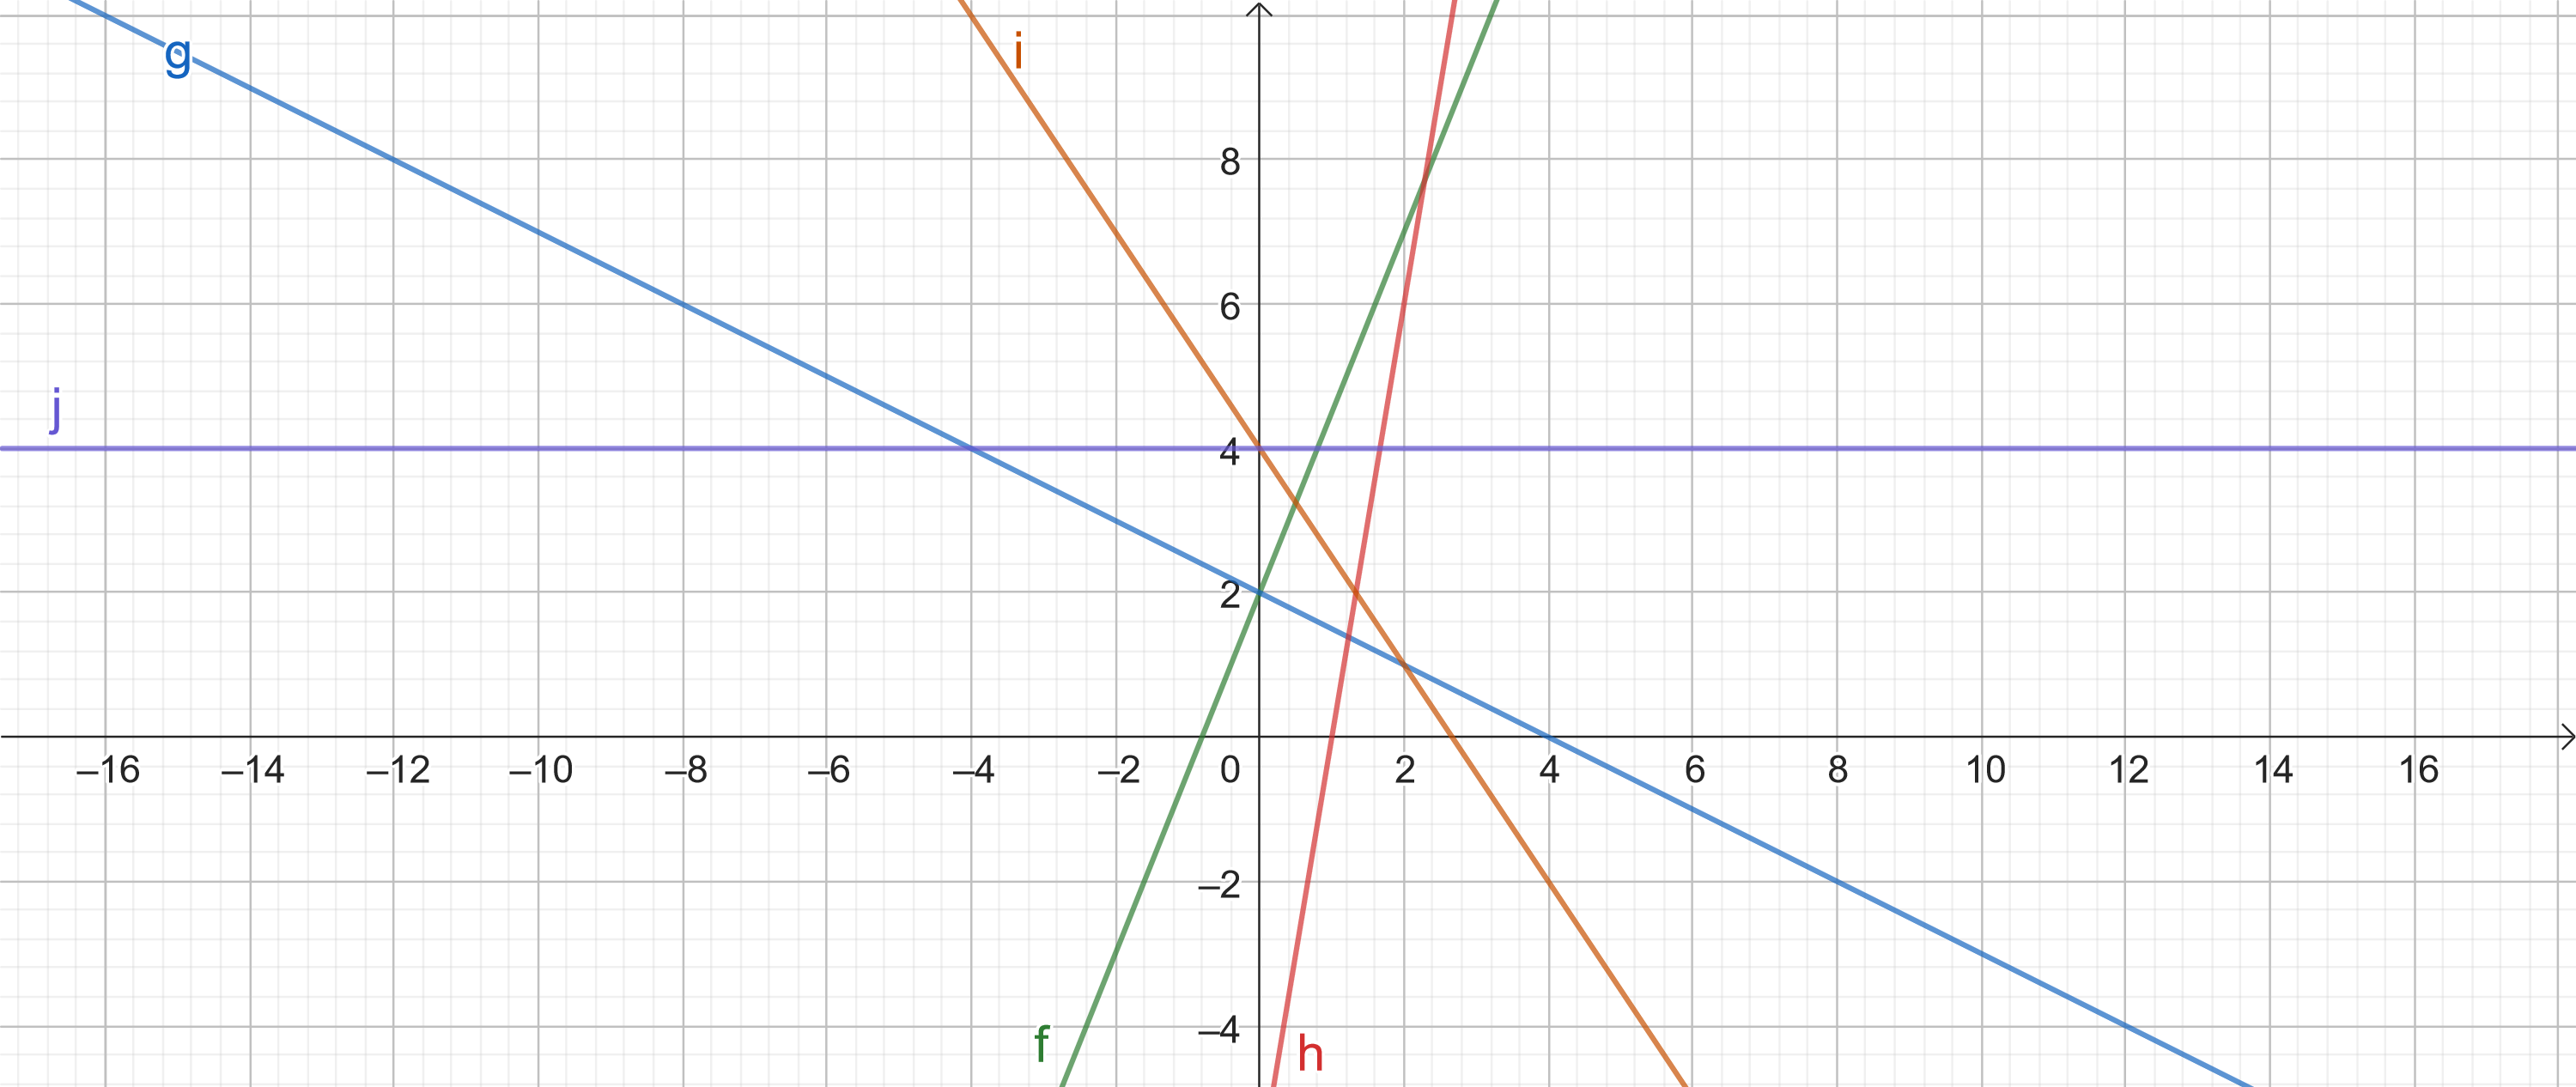
\includegraphics[width=\textwidth]{Exemples.png}
\end{center}

Nous avons représenté la courbe représentative de cinq fonctions affines : $f, g, h, i$ et $j$.

\section{Départ}
Pour chacun des critères suivants, sélectionner quelle(s) fonction(s) rempli(ssen)t le mieux ce critère.

\begin{enumerate}
\item La fonction est croissante :
\item La fonction est décroissante :
\item La fonction est constante :
\item La fonction a la plus petite ordonnée à l'origine :
\item La fonction a la plus grande pente :
\item La fonction passe par le point de coordonnées $(4,0)$ :
\item La fonction admet des images identiques à celles de $f$ en certains antécédents :
\item La fonction admet des images supérieures ou égales à celles de $j$ sur tout antécédent négatif :
\end{enumerate}

\section{Plus difficile ?}
Pour chacun des critères suivants, dessiner la courbe représentative d'une fonction affine vérifiant ce critère :
\begin{enumerate}
\item La fonction a la même pente que la fonction $i$.
\item La fonction passe par le point $(0,6)$.
\item La fonction a la même ordonnée à l'origine que $j$. 
\end{enumerate}
\end{document}